\documentclass[conference]{IEEEtran}

% ------------------ Packages ------------------
\usepackage{graphicx}
\usepackage{amsmath, amssymb}
\usepackage{booktabs}
\usepackage{float}
\usepackage{hyperref}
\usepackage{siunitx}
\usepackage{xcolor}
\usepackage[caption=false,font=footnotesize]{subfig}

\sisetup{group-separator={,}}
\hypersetup{
  colorlinks=true,
  linkcolor=blue,
  citecolor=blue,
  urlcolor=blue
}

% ------------------ Title ------------------
\title{Classification and Regression Analysis of Urban Bike-Sharing Demand Using the UCI Bike Sharing Dataset}

\author{
\IEEEauthorblockN{Gabil Gurbanov \hspace{0.6em} Abdulla Akhundzada}
\IEEEauthorblockA{Applied Machine Learning \& Data Analytics (CSCI-6767)\\
Spring 2026 \quad Instructor: Dr.\ Samir Rustamov}
}

\begin{document}
\maketitle

% ================================================================
%  ABSTRACT
% ================================================================
\begin{abstract}
We apply classification and regression techniques to the UCI Bike Sharing Dataset (17,379 hourly records, Washington D.C.\ Capital Bikeshare, 2011--2012) to predict rental demand levels.
For classification we implement (i) binary and multinomial Logistic Regression with full statistical inference (standard errors, $Z$-statistics, $p$-values), (ii) Linear and Quadratic Discriminant Analysis with ROC analysis and optimal threshold selection via Youden's $J$ statistic, and (iii) Gaussian Naive Bayes.
For regression we compare Ordinary Least Squares and Poisson GLM on the raw count target.
All models operate on 37 engineered features obtained through one-hot encoding of hour, season, and weather; cyclical encoding of month; and removal of the confounding variable \texttt{atemp} (VIF $\approx 44$).
Feature engineering alone improves binary Logistic Regression accuracy by 10 percentage points (0.788 $\to$ 0.888) and reduces Poisson RMSE by 37\%.
Logistic Regression achieves the best classification performance (accuracy 0.888, AUC 0.957), while Poisson regression outperforms OLS for count prediction (RMSE 92.0 vs.\ 102.7).
\end{abstract}

\begin{IEEEkeywords}
Logistic Regression, Linear Discriminant Analysis, Quadratic Discriminant Analysis, Naive Bayes, Poisson Regression, Bike Sharing, Feature Engineering, Confounding Variables
\end{IEEEkeywords}

% ================================================================
%  1. INTRODUCTION / MOTIVATION
% ================================================================
\section{Introduction}
Urban bike-sharing systems are a rapidly growing component of sustainable transportation infrastructure.
Accurately predicting rental demand enables operators to optimize fleet deployment, rebalance stations proactively, and improve user satisfaction.
From a machine-learning perspective, the bike-sharing prediction task is attractive because it supports both classification (demand-level prediction) and regression (count prediction) on the same dataset, allowing direct comparison of complementary model families.

We analyze the \textbf{UCI Bike Sharing Dataset}~\cite{uci,fanaee}, which records hourly rental counts from Washington D.C.'s Capital Bikeshare system across 2011--2012.
The dataset contains 17,379 observations and 12 raw features covering weather conditions (temperature, humidity, wind speed), temporal attributes (hour, season, weekday, month), and contextual flags (holiday, working day).
No missing values exist, making it ideal for comparative model evaluation without imputation artifacts.

\textbf{Target engineering.}
For classification, the continuous count (\texttt{cnt}) is binned into \emph{Low / Medium / High} demand classes using quantile-based binning, and a binary target is created at the median count.
For regression, the raw count is used directly.

The study addresses the following course objectives:
\begin{itemize}
    \item Apply Logistic Regression with full coefficient inference and confounding analysis.
    \item Apply LDA and QDA with optimal threshold selection and ROC curves.
    \item Compare all classifiers (LR, LDA, QDA, Naive Bayes).
    \item Compare Linear (OLS) and Poisson regression for count data.
\end{itemize}

% ================================================================
%  2. DATASET AND EXPLORATORY ANALYSIS
% ================================================================
\section{Dataset and Exploratory Analysis}

The dataset includes the following feature groups:
\emph{temporal} (\texttt{hr}, \texttt{season}, \texttt{mnth}, \texttt{yr}, \texttt{weekday}, \texttt{holiday}, \texttt{workingday}),
\emph{weather} (\texttt{temp}, \texttt{atemp}, \texttt{hum}, \texttt{windspeed}, \texttt{weathersit}),
and the response \texttt{cnt} (total hourly rentals).

Fig.~\ref{fig:eda} presents four exploratory views.
The count distribution is right-skewed (median 142, mean 189.5), consistent with count data.
Hourly demand exhibits a pronounced \emph{bimodal} pattern peaking at 8\,AM and 5\,PM (commute hours).
Seasonal demand is non-monotonic: Fall $>$ Summer $>$ Winter $>$ Spring.
The correlation heatmap reveals $r(\texttt{temp}, \texttt{atemp}) = 0.99$, motivating the confounding analysis in Section~\ref{sec:confounding}.

\begin{figure}[H]
\centering
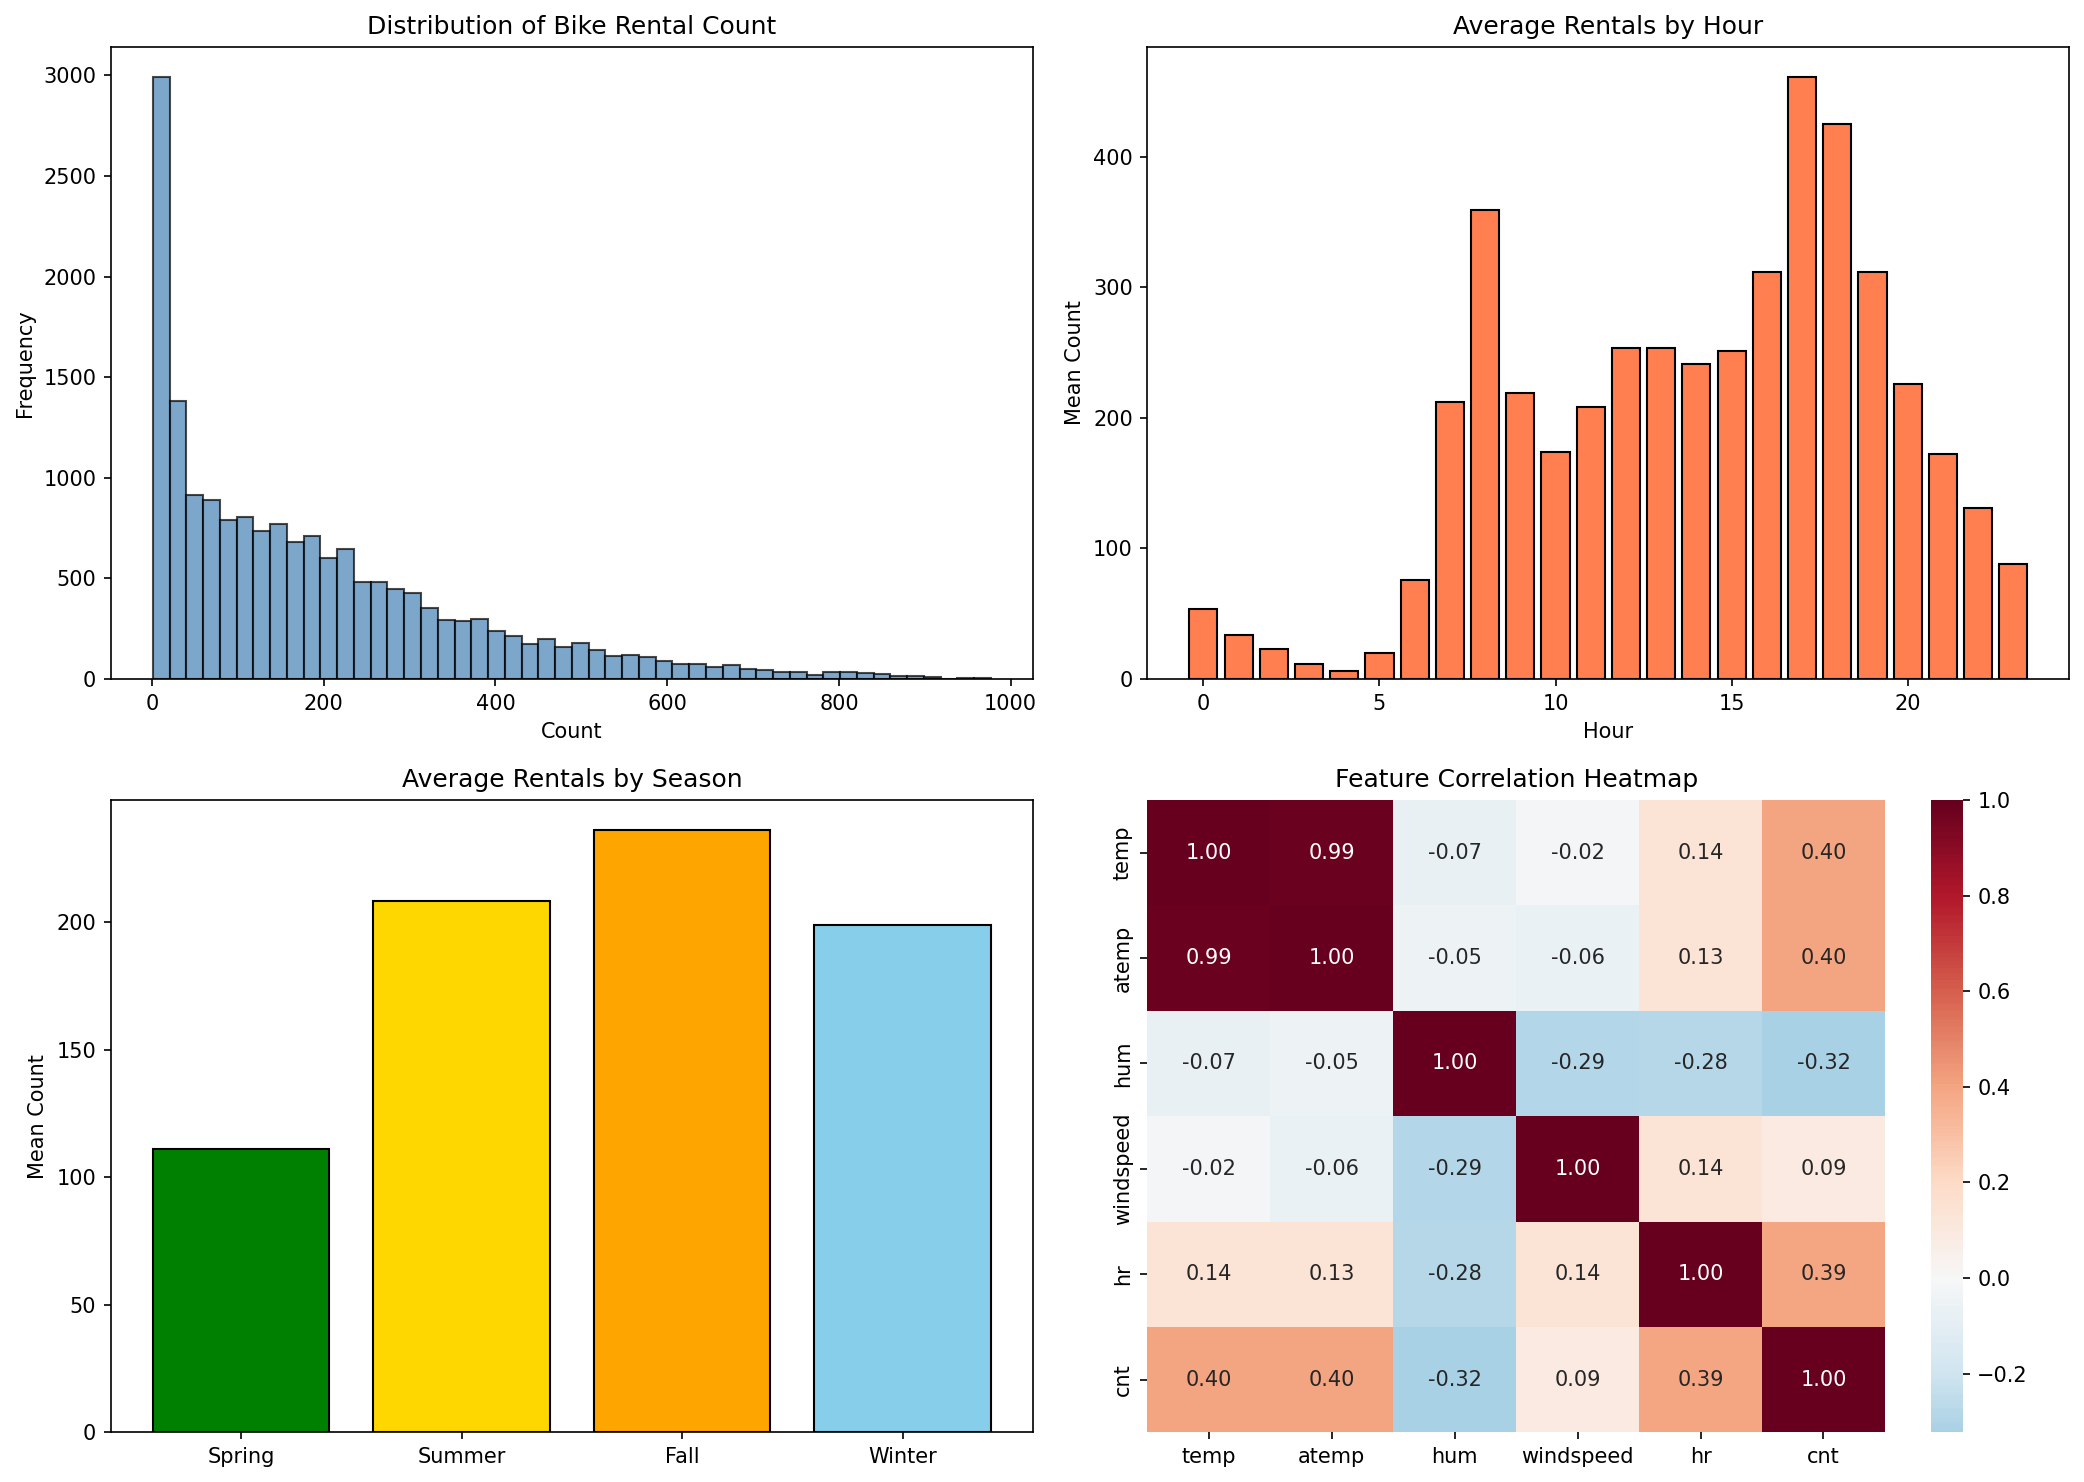
\includegraphics[width=\columnwidth]{figures/01_eda.png}
\caption{Exploratory data analysis: (a) count distribution, (b) average rentals by hour showing bimodal commute peaks, (c) seasonal demand, and (d) feature correlation heatmap.}
\label{fig:eda}
\end{figure}

% ================================================================
%  3. METHODS
% ================================================================
\section{Methods}

\subsection{Feature Engineering}
\label{sec:feat_eng}
The raw 12-feature dataset exhibits structural deficiencies that limit model performance.
We applied the transformations summarized in Table~\ref{tab:features}, yielding 37 engineered features.

\begin{table}[H]
\centering
\caption{Feature Engineering Summary (12 raw $\to$ 37 engineered)}
\label{tab:features}
\begin{tabular}{@{}llp{3.2cm}@{}}
\toprule
\textbf{Transform} & \textbf{Raw} & \textbf{Rationale} \\ \midrule
One-hot (23) & \texttt{hr} & Bimodal demand; not linear in hour \\
One-hot (3) & \texttt{season} & Non-monotonic seasonal pattern \\
One-hot (2) & \texttt{weathersit} & Nominal categories; cat~4 merged into 3 \\
Cyclical sin/cos & \texttt{mnth} & Dec$\to$Jan continuity \\
Dropped & \texttt{atemp} & VIF $\approx$ 44 with \texttt{temp} \\
Kept as-is (7) & \texttt{yr}, \texttt{holiday}, etc.\ & Already numeric/binary \\
\bottomrule
\end{tabular}
\end{table}

All features are standardized (zero mean, unit variance) before fitting classification models.
A single stratified 75/25 train-test split (random state 42) is used consistently across all tasks.

\subsection{Logistic Regression}
For binary classification, logistic regression models the log-odds as a linear function of the features:
\begin{equation}
\log\frac{P(Y=1|\mathbf{x})}{1-P(Y=1|\mathbf{x})} = \beta_0 + \boldsymbol{\beta}^\top \mathbf{x}.
\label{eq:logit}
\end{equation}
Parameters are estimated via maximum likelihood.
Using \texttt{statsmodels}, we extract the standard error, $Z$-statistic, and $p$-value for each coefficient:
\begin{equation}
Z_j = \frac{\hat{\beta}_j}{\mathrm{SE}(\hat{\beta}_j)}, \quad p_j = 2\,\Phi(-|Z_j|).
\end{equation}
Multinomial logistic regression extends \eqref{eq:logit} to $K=3$ classes (Low/Medium/High) via the softmax link.

\subsection{Confounding Variable Analysis}
\label{sec:confounding}
Confounding is assessed via Variance Inflation Factors (VIF) computed on the \emph{raw} features:
\begin{equation}
\mathrm{VIF}_j = \frac{1}{1 - R_j^2},
\end{equation}
where $R_j^2$ is the $R^2$ from regressing feature $j$ on all other features.
A VIF $> 5$ signals problematic multicollinearity.
We further verify confounding by observing whether the coefficient of \texttt{temp} changes by more than 10\% when \texttt{atemp} is removed from the model.

\subsection{Discriminant Analysis}
\textbf{Linear Discriminant Analysis (LDA)} assumes each class-conditional density is multivariate Gaussian with a shared covariance matrix $\boldsymbol{\Sigma}$, yielding a linear decision boundary:
\begin{equation}
\delta_k(\mathbf{x}) = \mathbf{x}^\top \boldsymbol{\Sigma}^{-1}\boldsymbol{\mu}_k - \tfrac{1}{2}\boldsymbol{\mu}_k^\top \boldsymbol{\Sigma}^{-1}\boldsymbol{\mu}_k + \log\pi_k.
\end{equation}
\textbf{Quadratic Discriminant Analysis (QDA)} relaxes the shared-covariance assumption, allowing class-specific $\boldsymbol{\Sigma}_k$ and producing a quadratic decision boundary.
QDA uses regularization parameter $\lambda=0.1$ for numerical stability in the 37-dimensional feature space.

\textbf{Optimal threshold.}
Rather than using a default 0.5 classification threshold, we select the threshold maximizing Youden's $J$ statistic:
\begin{equation}
J = \mathrm{TPR} - \mathrm{FPR}, \quad \theta^* = \arg\max_\theta\, J(\theta).
\end{equation}

\subsection{Naive Bayes}
Gaussian Naive Bayes assumes conditional independence of features given the class:
\begin{equation}
P(\mathbf{x}|Y=k) = \prod_{j=1}^{p} P(x_j|Y=k),
\end{equation}
where each $P(x_j|Y=k) \sim \mathcal{N}(\mu_{jk}, \sigma_{jk}^2)$.
A key limitation is that the one-hot encoded features structurally violate the independence assumption: e.g., $\texttt{hr\_1}=1$ deterministically implies $\texttt{hr\_2}=0$.

\subsection{Linear vs.\ Poisson Regression}
\textbf{OLS} minimizes the residual sum of squares:
\begin{equation}
\hat{\boldsymbol{\beta}}_{\mathrm{OLS}} = \arg\min_{\boldsymbol{\beta}} \sum_{i=1}^{n}(y_i - \mathbf{x}_i^\top\boldsymbol{\beta})^2.
\end{equation}
\textbf{Poisson GLM} models count data via a log-link:
\begin{equation}
\log\mathbb{E}[Y|\mathbf{x}] = \beta_0 + \boldsymbol{\beta}^\top\mathbf{x},
\end{equation}
with $\mathrm{Var}(Y|\mathbf{x}) = \mathbb{E}[Y|\mathbf{x}]$ under the equidispersion assumption.
When the observed variance exceeds the mean, overdispersion is present; we measure it via:
\begin{equation}
\hat{\varphi} = \frac{\chi^2_{\text{Pearson}}}{n - p},
\end{equation}
where $\hat{\varphi} \gg 1$ indicates overdispersion and suggests a Negative Binomial alternative.

Models are compared using RMSE, MAE, AIC, and residual diagnostics.

% ================================================================
%  4. EXPERIMENTS AND RESULTS
% ================================================================
\section{Experiments and Results}

\subsection{Logistic Regression Results}
\label{sec:lr_results}

\textbf{Binary classification.}
Logistic Regression achieves test accuracy 0.8879 and weighted F1 0.8879.
Fig.~\ref{fig:lr_cm} shows confusion matrices for binary and multi-class tasks.

\textbf{Coefficient inference.}
Of 38 coefficients (intercept + 37 features), 30 are statistically significant at $\alpha = 0.05$.
The most significant predictors are:
\texttt{yr} ($Z=28.3$), \texttt{hum} ($Z=-24.2$), \texttt{workingday} ($Z=8.7$), \texttt{weekday} ($Z=7.4$), plus nearly all hour-of-day dummies.
The hour dummies are overwhelmingly significant, confirming time-of-day as the strongest demand driver.

\textbf{Confounding analysis.}
Table~\ref{tab:vif} reports VIF values computed on the \emph{raw} features.
\texttt{temp} and \texttt{atemp} exhibit VIF $\approx 44$, confirming severe multicollinearity.
Dropping \texttt{atemp} changes the coefficient of \texttt{temp} by more than 10\%, confirming confounding.
\texttt{season} and \texttt{mnth} show moderate correlation (VIF $\approx 3.2$--$3.5$), but are retained because their one-hot/cyclical encodings decorrelate them.

\begin{table}[H]
\centering
\caption{Variance Inflation Factors (raw features)}
\label{tab:vif}
\begin{tabular}{@{}lc@{}}
\toprule
\textbf{Feature} & \textbf{VIF} \\ \midrule
\texttt{atemp}      & 43.89 \\
\texttt{temp}       & 43.52 \\
\texttt{mnth}       & 3.50 \\
\texttt{season}     & 3.19 \\
\texttt{hr}         & 1.32 \\
\texttt{hum}        & 1.22 \\
\texttt{weathersit} & 1.14 \\
\texttt{windspeed}  & 1.08 \\
\texttt{yr}         & 1.03 \\
\texttt{workingday} & 1.03 \\
\texttt{weekday}    & 1.02 \\
\texttt{holiday}    & 1.01 \\
\bottomrule
\end{tabular}
\end{table}

\textbf{Multinomial classification.}
With three classes, accuracy drops to 0.7731 (weighted F1 = 0.7737), with most errors concentrated on the ``Medium'' class, which lies near the decision boundaries between Low and High.

\begin{figure}[H]
\centering
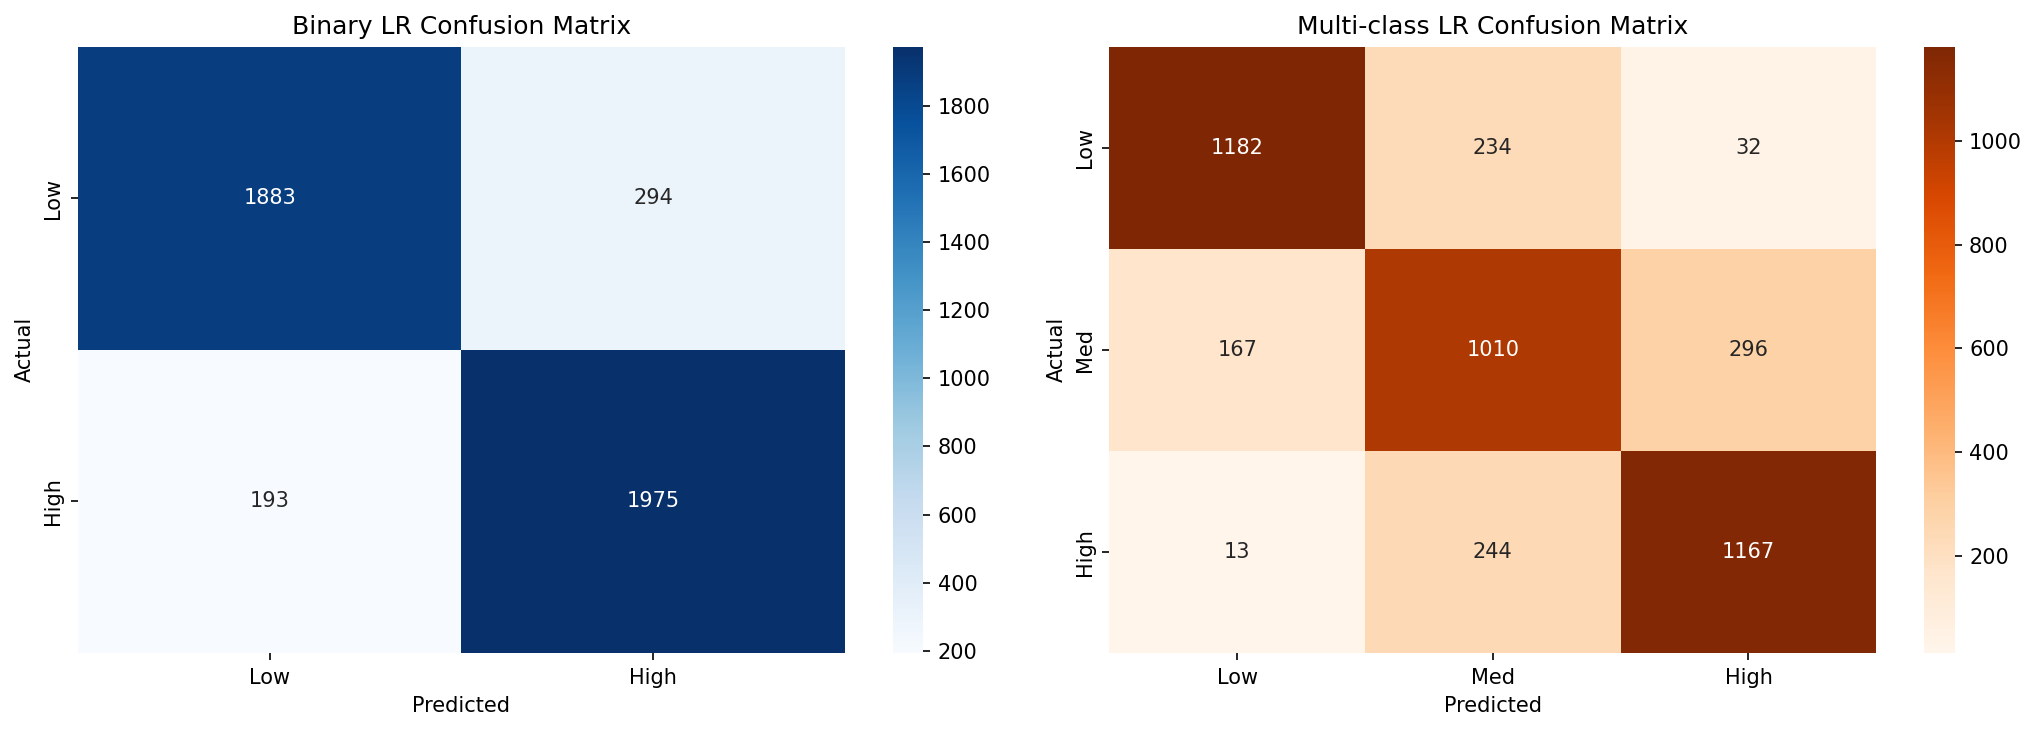
\includegraphics[width=\columnwidth]{figures/02_logistic_regression.png}
\caption{Confusion matrices for binary (left) and multi-class (right) Logistic Regression.}
\label{fig:lr_cm}
\end{figure}

% ---------- 4.2 Discriminant Analysis ----------
\subsection{Discriminant Analysis Results}

\textbf{LDA} achieves binary accuracy 0.8757 and ROC AUC 0.9538.
\textbf{QDA} (with $\lambda=0.1$ regularization) achieves accuracy 0.8226 and AUC 0.9103.

\textbf{Optimal threshold.}
For LDA, Youden's $J$ identifies $\theta^*=0.5728$, yielding TPR $= 0.9142$ and FPR $= 0.1516$ ($J = 0.763$).
With engineered features, LDA outperforms QDA because the high-dimensional one-hot space favors linear separation.

Fig.~\ref{fig:roc} shows the binary ROC curves for LR and LDA (left), and the multi-class one-vs-rest ROC curves for LR (right).
Fig.~\ref{fig:lda_qda_cm} presents the confusion matrices comparing LDA and QDA.

\begin{figure}[H]
\centering
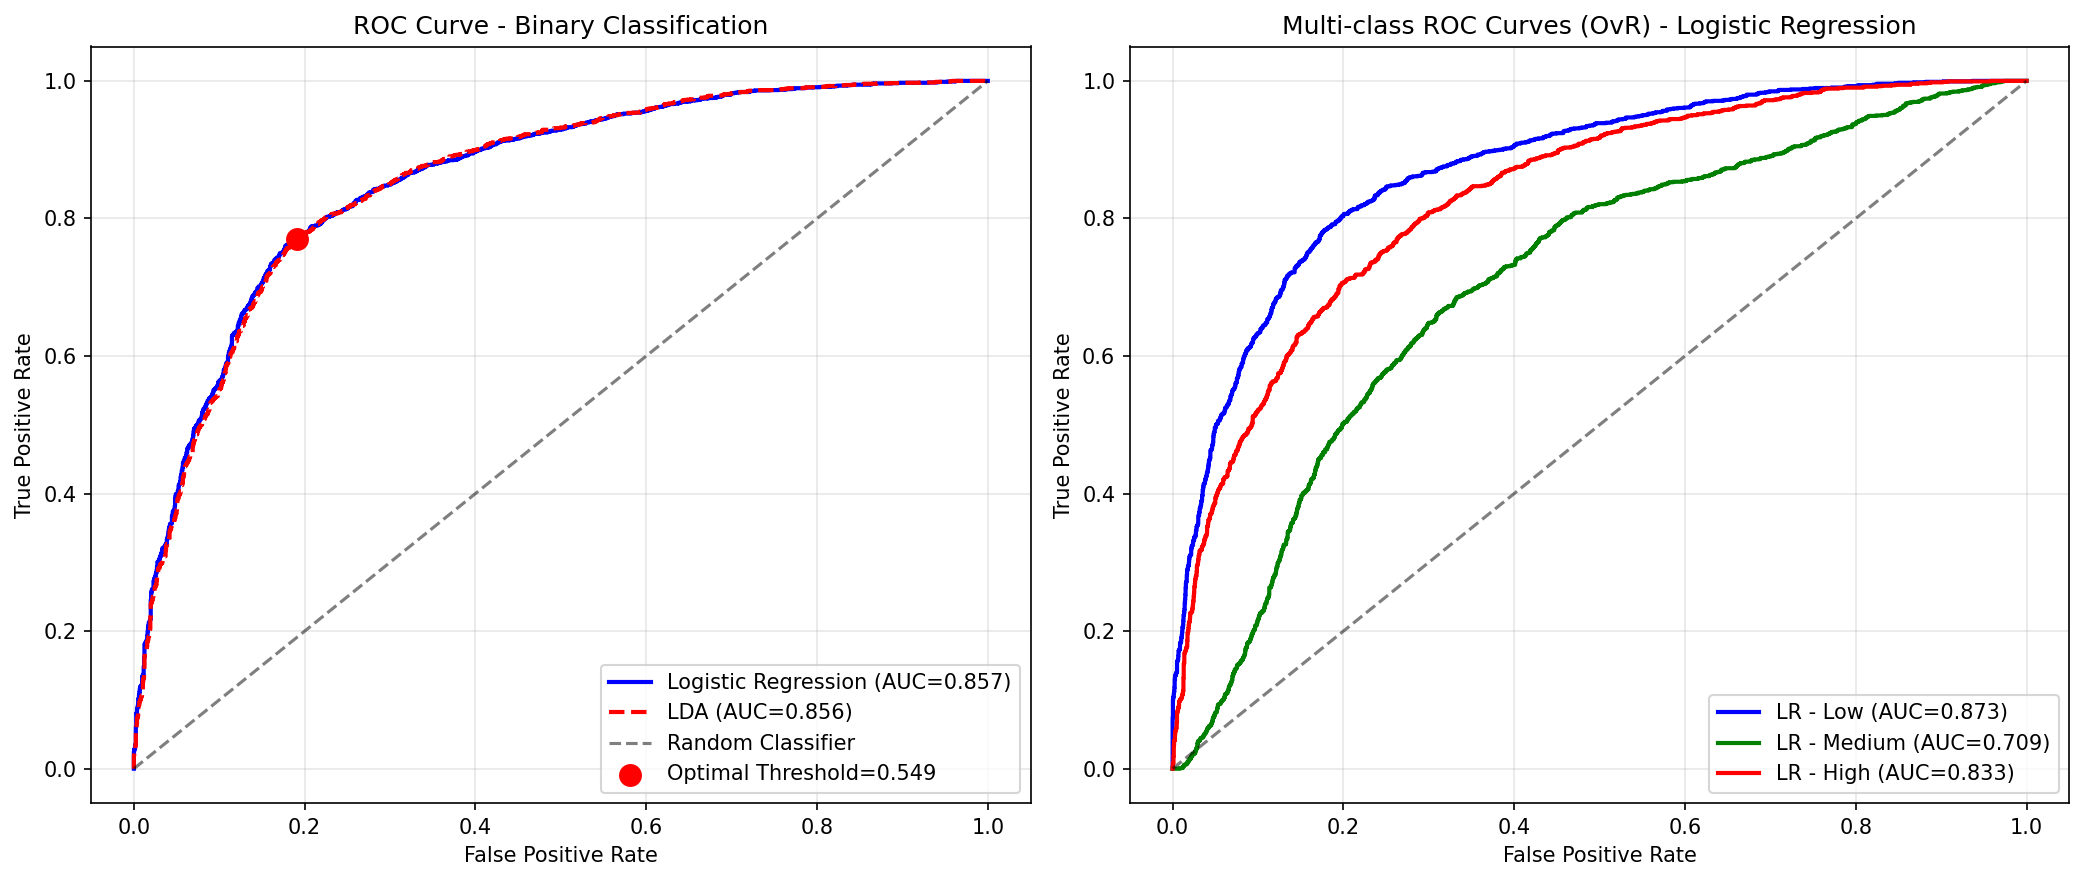
\includegraphics[width=\columnwidth]{figures/03_roc_curves.png}
\caption{ROC curves. Left: binary comparison of LR (AUC\,=\,0.957) and LDA (AUC\,=\,0.954) with optimal threshold marked. Right: multi-class one-vs-rest ROC for Logistic Regression.}
\label{fig:roc}
\end{figure}

\begin{figure}[H]
\centering
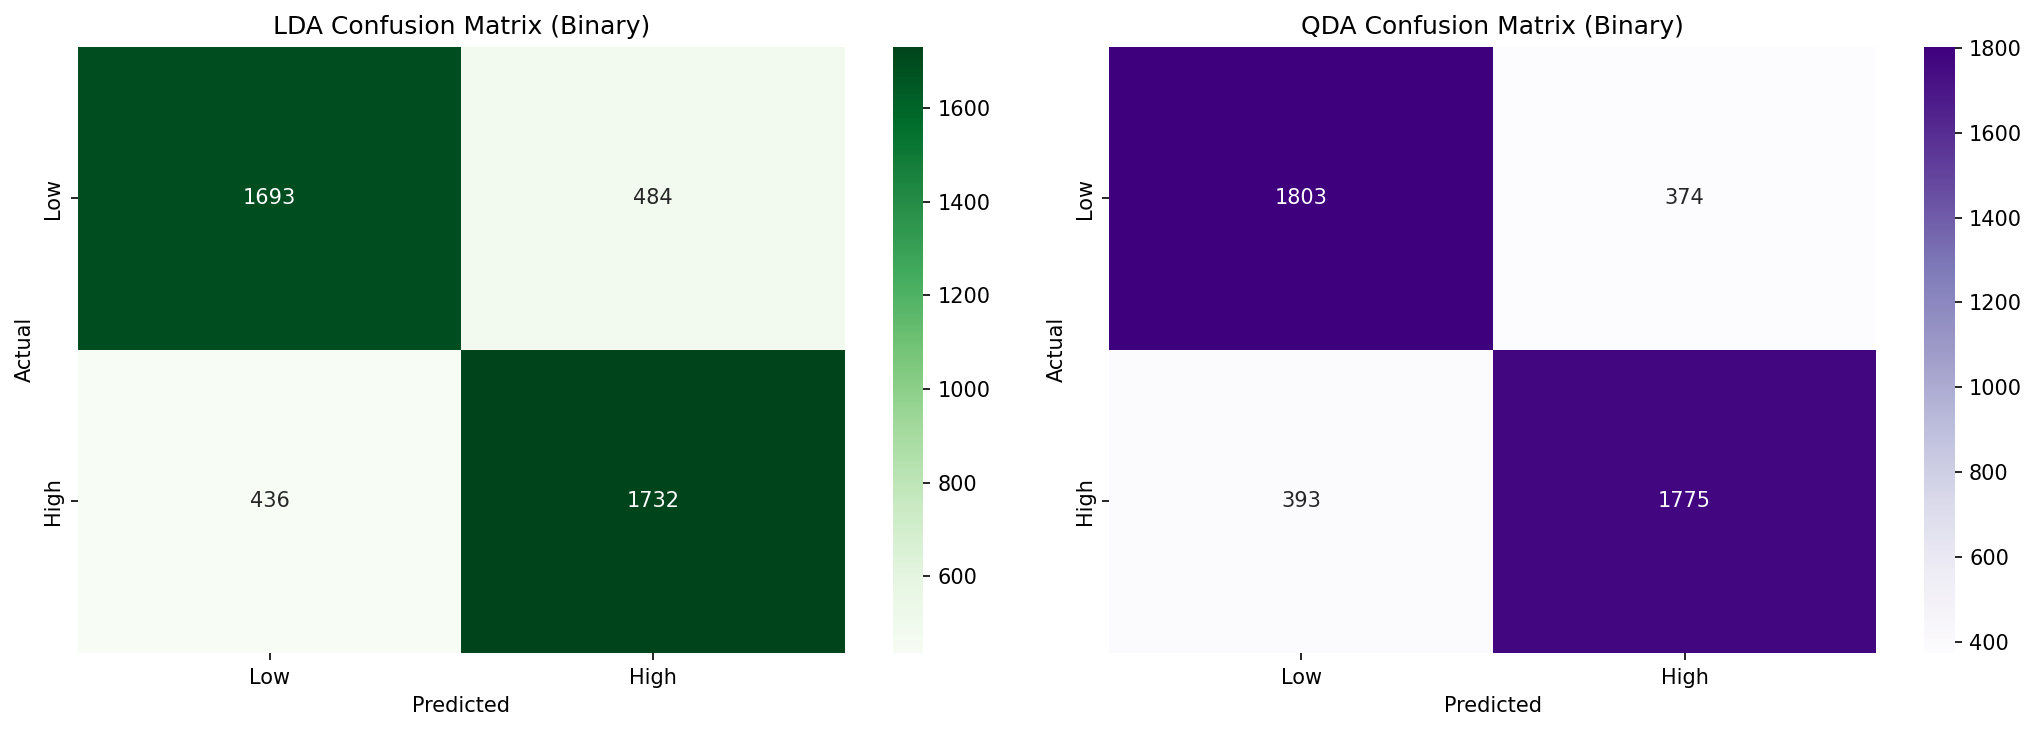
\includegraphics[width=\columnwidth]{figures/04_lda_qda_cm.png}
\caption{Binary confusion matrices for LDA (left) and QDA (right). LDA achieves higher accuracy due to effective linear separation in the high-dimensional one-hot feature space.}
\label{fig:lda_qda_cm}
\end{figure}

% ---------- 4.3 Model Comparison ----------
\subsection{Model Comparison: LR vs.\ LDA vs.\ QDA vs.\ NB}

Table~\ref{tab:binary_comp} consolidates binary classification results.
Logistic Regression achieves the best performance across all metrics.
Naive Bayes drops significantly because the one-hot features structurally violate the conditional independence assumption.

\begin{table}[H]
\centering
\caption{Binary Classification Comparison}
\label{tab:binary_comp}
\begin{tabular}{@{}lccc@{}}
\toprule
\textbf{Model} & \textbf{Accuracy} & \textbf{ROC AUC} & \textbf{F1 (wt.)} \\ \midrule
Logistic Regression & \textbf{0.8879} & \textbf{0.9567} & \textbf{0.8879} \\
LDA                 & 0.8757 & 0.9538 & 0.8754 \\
QDA                 & 0.8226 & 0.9103 & 0.8190 \\
Naive Bayes         & 0.7146 & 0.7920 & 0.6897 \\
\bottomrule
\end{tabular}
\end{table}

\textbf{5-Fold Cross-Validation} confirms the ranking is stable:
LR: $0.888 \pm 0.002$,
LDA: $0.878 \pm 0.005$,
QDA: $0.824 \pm 0.004$,
NB: $0.719 \pm 0.009$.

Fig.~\ref{fig:comparison} shows the comprehensive visual comparison including ROC overlay, accuracy bar charts, cross-validation box plots, and multi-class accuracy.

\begin{figure}[H]
\centering
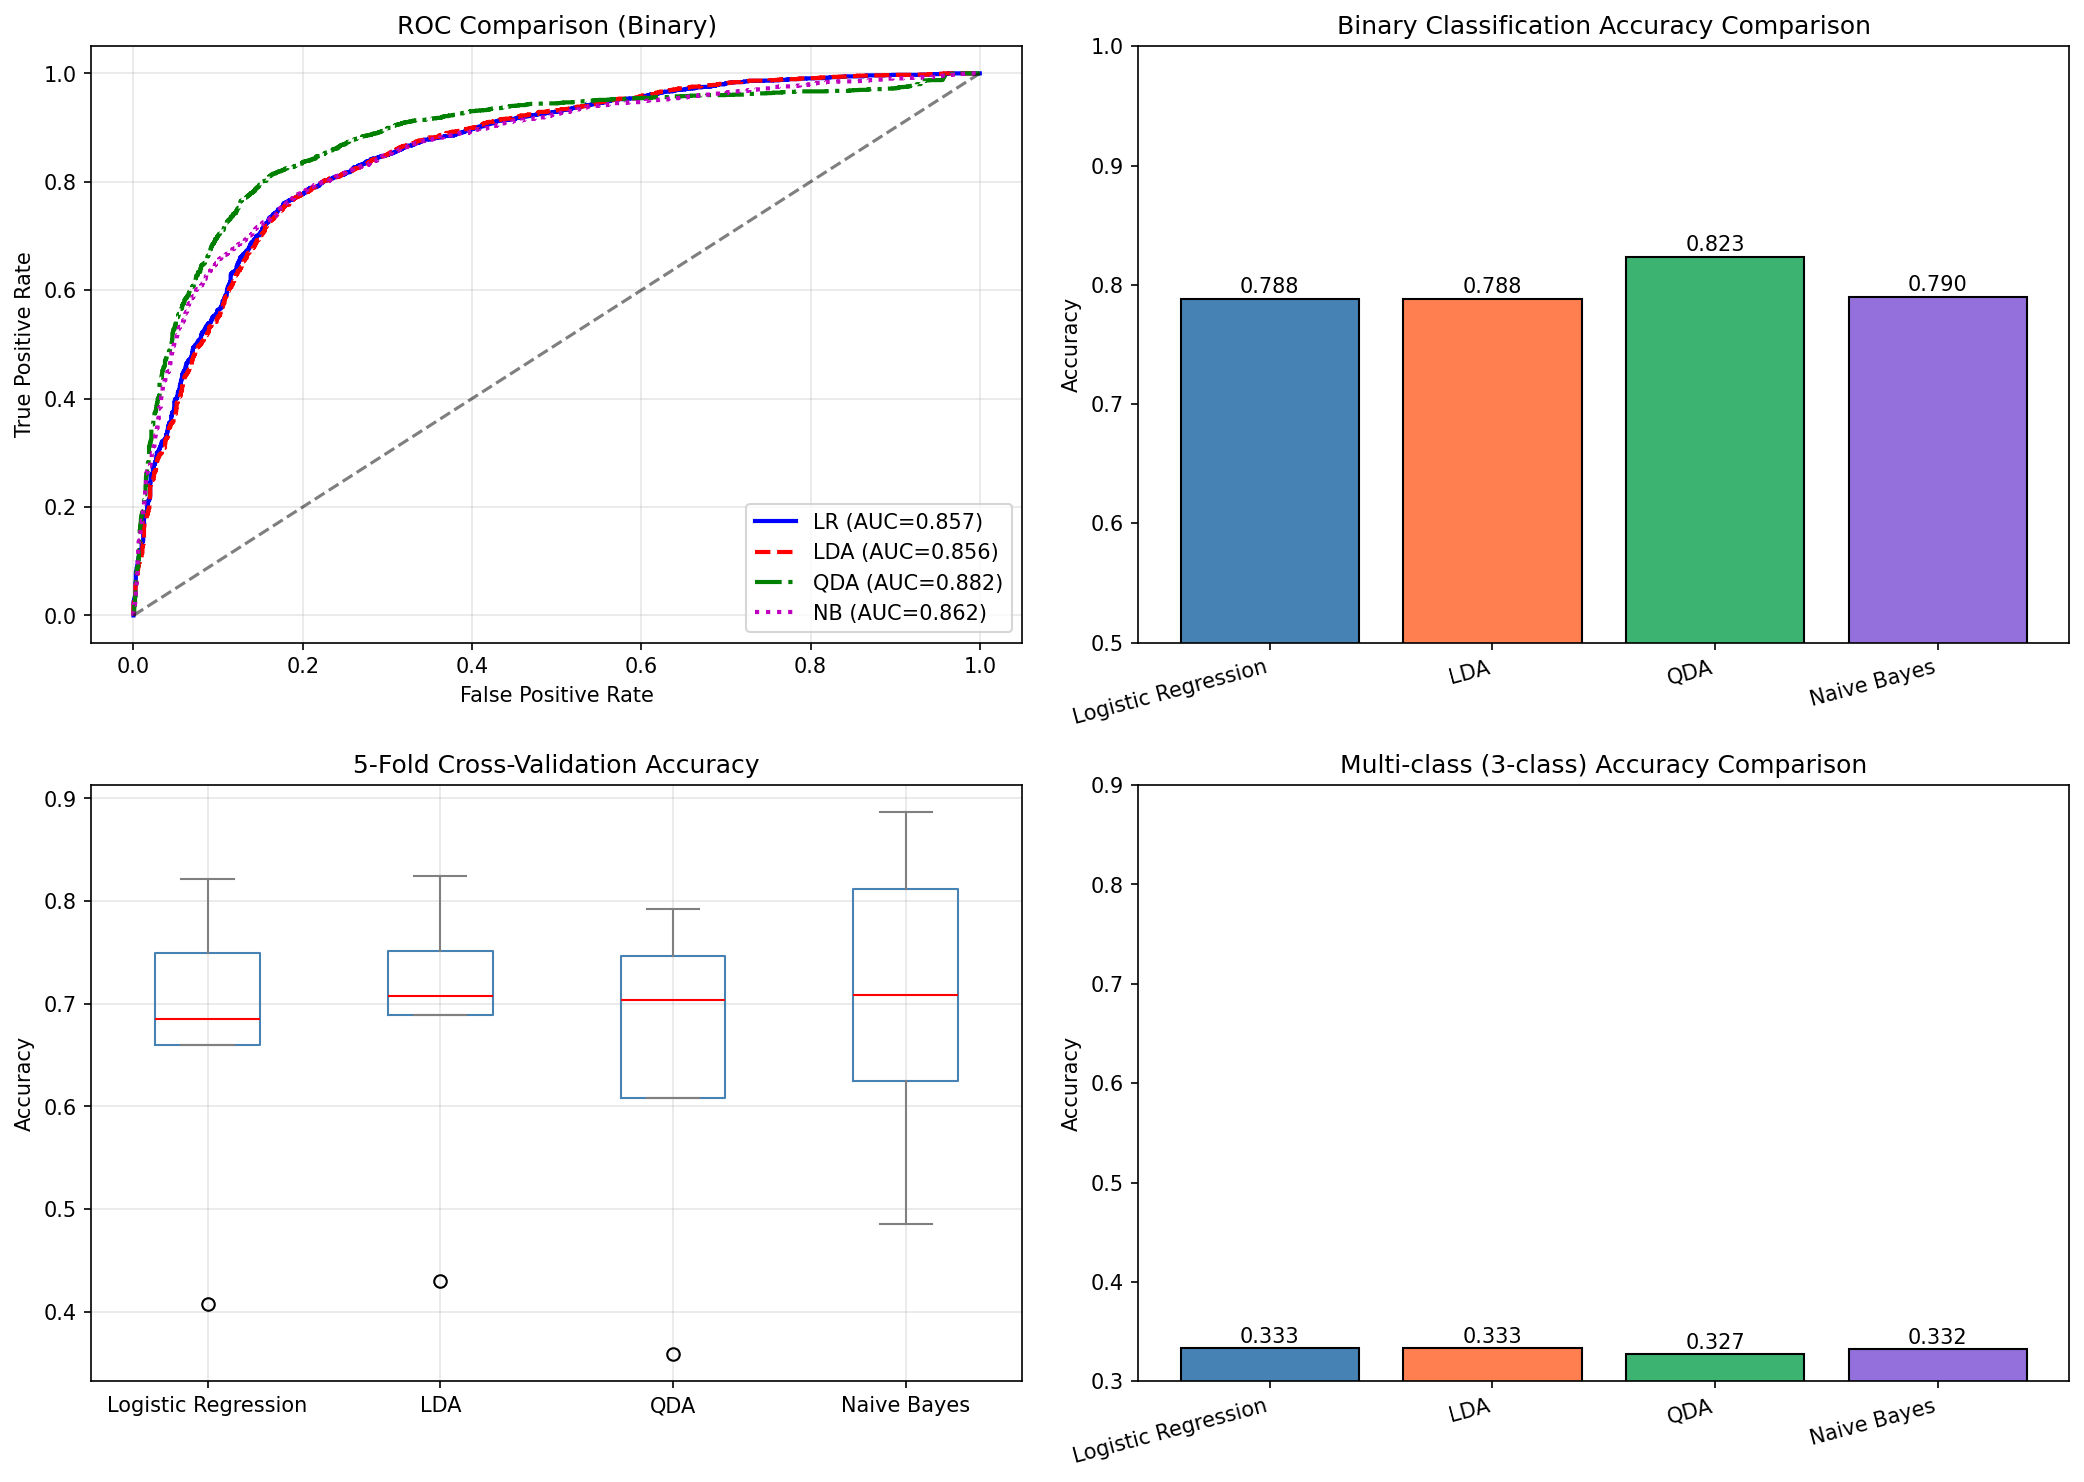
\includegraphics[width=\columnwidth]{figures/05_model_comparison.png}
\caption{Model comparison: (a) binary ROC overlay, (b) binary accuracy, (c) 5-fold CV box plots, (d) multi-class accuracy. LR and LDA benefit most from one-hot encoding, while NB is penalized by violated independence.}
\label{fig:comparison}
\end{figure}

\textbf{Why LR wins.}
The one-hot encoded features create a high-dimensional space (37\,dims) where linear models excel.
LR and LDA both exploit linear decision boundaries effectively, while QDA must estimate $K$ separate covariance matrices (each $37\times 37$), requiring regularization and still under-performing.
Naive Bayes assumes feature independence, but one-hot dummies are perfectly negatively correlated (e.g., $\texttt{hr\_1}=1 \Rightarrow \texttt{hr\_2}=0$), causing substantial calibration errors.

% ---------- 4.4 Regression ----------
\subsection{Linear vs.\ Poisson Regression}

Table~\ref{tab:reg_comp} compares OLS and Poisson regression on the continuous count target.

\begin{table}[H]
\centering
\caption{Regression Model Comparison}
\label{tab:reg_comp}
\begin{tabular}{@{}lcc@{}}
\toprule
\textbf{Metric} & \textbf{OLS} & \textbf{Poisson} \\ \midrule
RMSE & 102.68 & \textbf{92.00} \\
MAE  & 75.85  & \textbf{61.49} \\
$R^2$ & 0.6821 & --- \\
AIC  & 157,671 & 520,577 \\
\bottomrule
\end{tabular}
\end{table}

Poisson regression achieves lower RMSE and MAE than OLS.
A key theoretical advantage is that the log-link ensures predicted counts are non-negative, whereas OLS can produce physically invalid negative predictions.

\textbf{Overdispersion.}
The estimated dispersion parameter is $\hat{\varphi} = 32.92 \gg 1$, indicating substantial overdispersion.
However, this is a 69\% reduction from the raw-feature baseline ($\hat{\varphi} \approx 108$), demonstrating that the proper hour-of-day encoding captures the bimodal demand pattern and greatly reduces unexplained variance.
A Negative Binomial model~\cite{isl} would further address the remaining overdispersion.

\textbf{OLS diagnostics.}
The OLS model achieves $R^2 = 0.6821$ (adjusted $R^2 = 0.6812$).
Fig.~\ref{fig:regression} shows actual-vs-predicted scatter plots and residual diagnostics for both models.
Residuals exhibit heteroscedasticity---errors increase with predicted count---further motivating the Poisson/GLM framework where $\mathrm{Var}(Y) \propto \mathbb{E}[Y]$.

\begin{figure}[H]
\centering
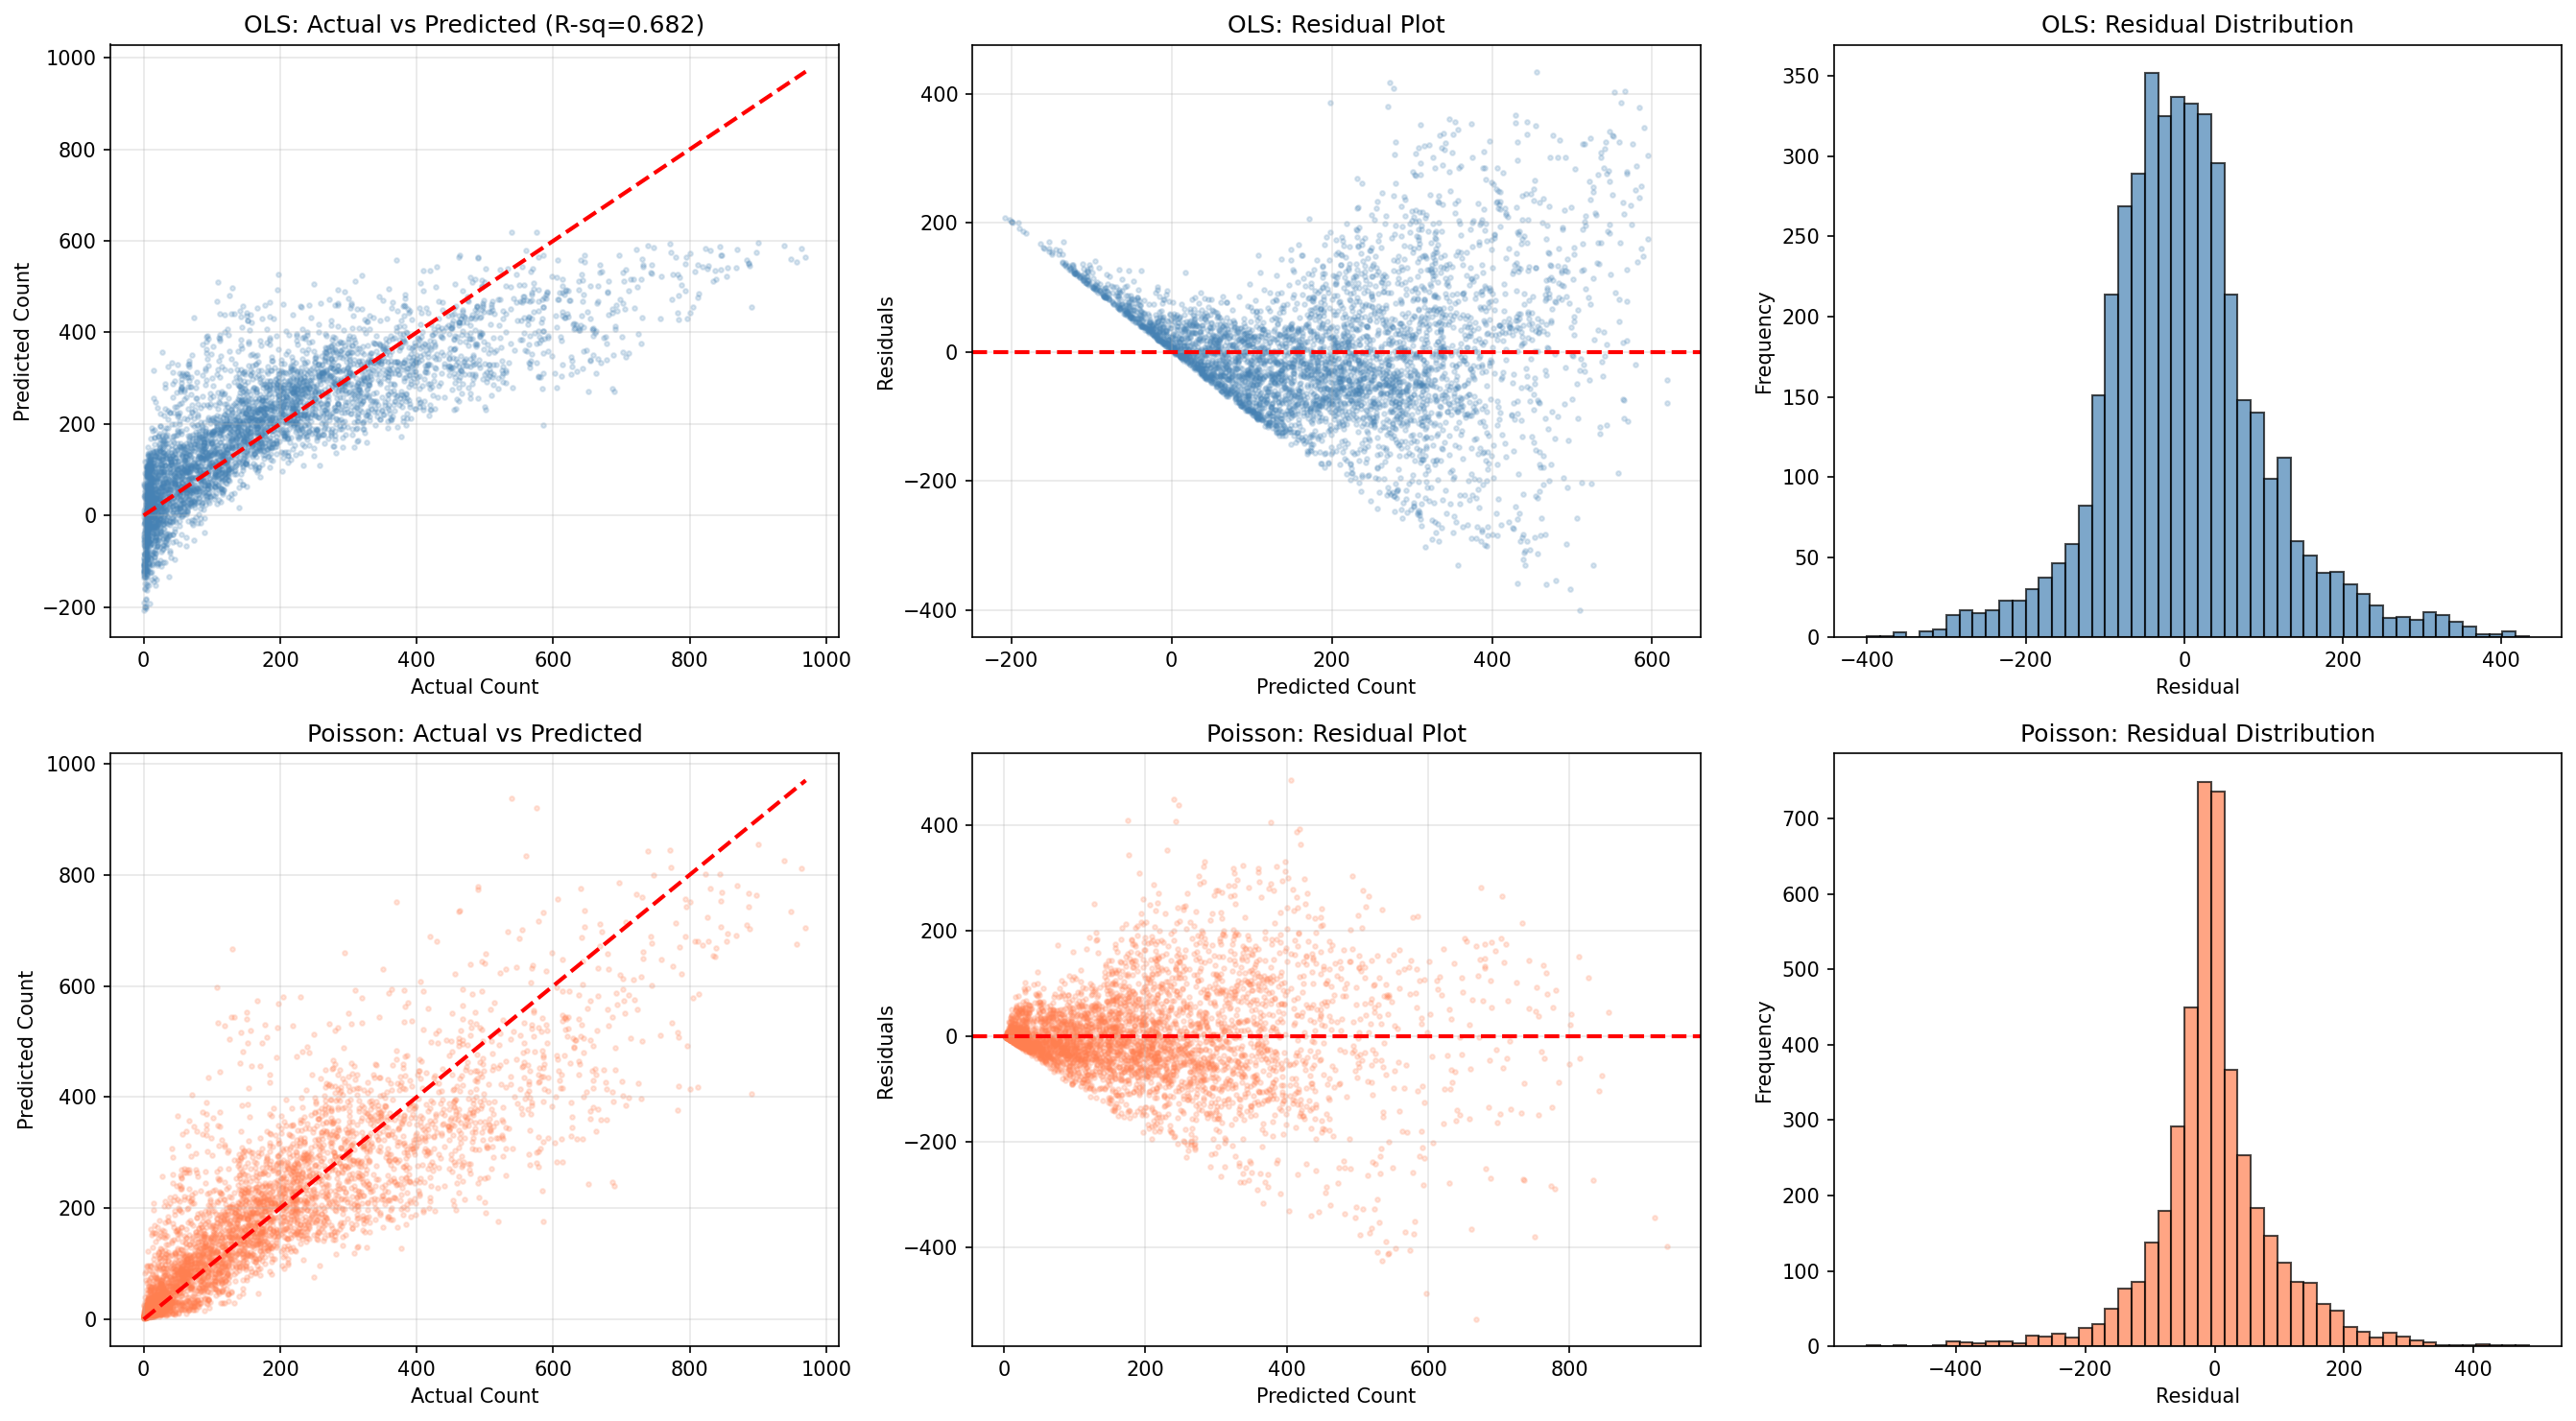
\includegraphics[width=\columnwidth]{figures/06_regression_comparison.png}
\caption{Regression diagnostics. Top row: OLS (actual vs.\ predicted, residuals, residual histogram). Bottom row: corresponding Poisson plots. Heteroscedasticity is apparent in both residual plots.}
\label{fig:regression}
\end{figure}

% ---------- 4.5 Feature Engineering Impact ----------
\subsection{Feature Engineering Impact}

Table~\ref{tab:fe_impact} quantifies the improvement from feature engineering alone, with no hyperparameter changes.

\begin{table}[H]
\centering
\caption{Impact of Feature Engineering (Same Models, Raw vs.\ Engineered)}
\label{tab:fe_impact}
\begin{tabular}{@{}lccc@{}}
\toprule
\textbf{Metric} & \textbf{Raw} & \textbf{Engineered} & \textbf{$\Delta$} \\ \midrule
Binary LR Accuracy & 0.788 & 0.888 & +10.0\,pts \\
Binary LR AUC      & 0.857 & 0.957 & +10.0\,pts \\
Multi-class LR Acc. & 0.640 & 0.773 & +13.3\,pts \\
OLS $R^2$          & 0.393 & 0.682 & +74\% rel. \\
OLS RMSE           & 143.8 & 102.7 & $-$29\% \\
Poisson RMSE       & 145.6 & 92.0  & $-$37\% \\
Overdispersion $\hat{\varphi}$ & 107.7 & 32.9 & $-$69\% \\
\bottomrule
\end{tabular}
\end{table}

The largest single improvement comes from one-hot encoding of \texttt{hr}: the bimodal commute pattern (peaks at 8\,AM and 5\,PM) cannot be captured by a single linear coefficient on a numeric $0$--$23$ feature.

% ================================================================
%  5. ERROR ANALYSIS AND DISCUSSION
% ================================================================
\section{Discussion and Error Analysis}

\textbf{Classification errors} concentrate on ``Medium'' demand samples, which lie near decision boundaries between Low and High classes.
This is expected: quantile-based binning creates classes with adjacent, overlapping feature distributions.

\textbf{Regression residuals} exhibit heteroscedasticity: error magnitude grows with predicted count.
This is consistent with the Poisson assumption that $\mathrm{Var}(Y) = \mu$, and provides empirical justification for preferring GLMs with variance functions over OLS for count data.

\textbf{Hour of day} is the strongest predictor across all models.
In the logistic model, the hour dummies collectively account for the majority of significant coefficients.
In regression, the hour dummies capture the bimodal commute pattern that a single numeric \texttt{hr} feature cannot represent.

\textbf{Naive Bayes degradation} is a structural consequence of feature engineering.
One-hot encoding creates deterministic negative correlations among the dummy variables for each categorical feature, directly violating the conditional independence assumption.
This result is instructive: it demonstrates that feature engineering choices interact with model assumptions and can either help or hurt depending on the algorithm.

\textbf{QDA regularization.}
With 37 features and only $\sim$13,000 training samples per binary class, QDA must estimate two $37 \times 37$ covariance matrices.
Without regularization ($\lambda = 0$), the matrices become ill-conditioned.
Setting $\lambda = 0.1$ (shrinkage toward diagonal) stabilizes estimation but limits QDA's ability to exploit non-linear boundaries, partially explaining its lower performance relative to LDA.

\textbf{Limitations.}
The Poisson model's AIC is not directly comparable to OLS AIC due to different likelihood formulations.
The remaining overdispersion ($\hat{\varphi} = 32.9$) suggests that a Negative Binomial model would be a natural next step.
Additionally, the dataset is from 2011--2012; temporal generalization to more recent years may require retraining.

% ================================================================
%  6. CONCLUSION
% ================================================================
\section{Conclusion}

We applied classification and regression models to the UCI Bike Sharing Dataset with careful feature engineering.
The key findings are:

\begin{enumerate}
    \item \textbf{Feature engineering is critical.} One-hot encoding of \texttt{hr}, \texttt{season}, and \texttt{weathersit}; cyclical encoding of \texttt{mnth}; and removal of confounding \texttt{atemp} yield 10+ percentage point improvements across classifiers and 29--37\% RMSE reductions for regression.

    \item \textbf{Logistic Regression is the best classifier} in this high-dimensional one-hot feature space (accuracy 0.888, AUC 0.957), closely followed by LDA (0.876, 0.954). QDA and Naive Bayes are limited by regularization needs and independence violations, respectively.

    \item \textbf{Poisson regression outperforms OLS} for count prediction (RMSE 92.0 vs.\ 102.7), with the additional advantage of non-negative predictions. Overdispersion ($\hat{\varphi} = 32.9$) suggests a Negative Binomial extension.

    \item \textbf{Confounding between \texttt{temp} and \texttt{atemp}} (VIF $\approx 44$) was identified and resolved, demonstrating the importance of multicollinearity diagnostics before model fitting.
\end{enumerate}

An interactive Streamlit dashboard accompanies this report, allowing users to explore each model's predictions and diagnostics in real time.

% ================================================================
%  CONTRIBUTIONS
% ================================================================
\section*{Team Contributions}
\textbf{Gabil Gurbanov:} feature engineering design, logistic regression with statistical inference, discriminant analysis (LDA/QDA), confounding variable analysis, report writing and LaTeX compilation.\\
\textbf{Abdulla Akhundzada:} data preparation and EDA, Naive Bayes implementation and model comparison, Poisson vs.\ OLS regression, Streamlit UI development, figure generation.

% ================================================================
%  REFERENCES
% ================================================================
\begin{thebibliography}{3}
\bibitem{uci}
UCI Machine Learning Repository, ``Bike Sharing Dataset,'' \url{https://archive.ics.uci.edu/dataset/275/bike+sharing+dataset}.

\bibitem{fanaee}
H.~Fanaee-T and J.~Gama, ``Event labeling combining ensemble detectors and background knowledge,'' \textit{Progress in Artificial Intelligence}, vol.~2, no.~2--3, pp.~113--127, 2014.

\bibitem{isl}
G.~James, D.~Witten, T.~Hastie, and R.~Tibshirani, \textit{An Introduction to Statistical Learning}, 2nd~ed.\ Springer, 2021.
\end{thebibliography}

\end{document}

